\chapter{Job scheduling}
\label{chap:refs}

Job scheduling allocates jobs to machines. There are many different variants of job scheduling, each with different constraints and assumptions. This thesis deals with three particular variants: JSSP, FJSP, and DJSP. This chapter defines each variant and discusses relevant graph representations and Markov Decision Process (MDP) formulations.

\section{Job-Shop Scheduling Problem}

The simplest variant of job scheduling called JSSP consists of a set of jobs $\mathcal{J}$ and a set of machines $\mathcal{M}$ \cite{YamadaNakanoJSSP}. Each job has an associated ordered sequence of operations $O_{ij}$ to be processed. Operation $\mathcal{O}_{ij}$ represents uninterrupted processing of job $J_i \in \mathcal{J}$ on machine $M_j \in \mathcal{M}$ with processing time $p_{ij}$. Each machine can process only one operation at a time. A schedule is a set of start times $S_{ij}$ for each operation $O_{ij}$ that satisfies these constraints. Completion times $C_{ij} = S_{ij} + p_{ij}$ denote the end of each operation. The JSSP solution is a schedule minimizing total makespan $C_\text{max} = \text{max}_{i,j} \{C_{ij}\}$ \cite{zhang2020learning}. An example of a JSSP instance with three jobs and three machines (3x3) is shown in table 1.1 \cite{YamadaNakanoJSSP}.
\begin{table}[htbp]
    Table 1.1: 3x3 example JSSP instance \cite{YamadaNakanoJSSP}\\
    \vspace{1mm}
    \begin{tabular}{cccc}
    \hline
    job & \multicolumn{3}{c}{Machine (processing time)} \\ \hline
    1   & 1 (3)             & 2 (3)             & 3 (3)            \\
    2   & 1 (2)             & 3 (3)             & 2 (4)            \\
    3   & 2 (3)             & 1 (2)             & 3 (1)            \\ \hline
    \end{tabular}
\end{table}\\
The Gantt-Chart is a convenient tool for visualizing schedules \cite{WILSON2003430}. An example of a solution for the 3x3 problem from Table 1.1 is shown in Figure 1.1.
\begin{center}
    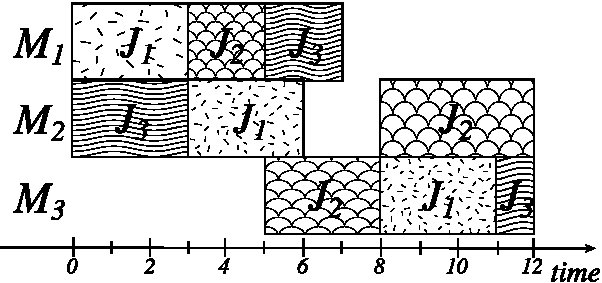
\includegraphics[width=0.8\linewidth]{images/gantt-charrt.pdf}\\
    Figure 1.1: Gantt-Chart of a solution for a 3x3 problem in table 1.1, reproduced from \cite{YamadaNakanoJSSP}
\end{center}

\section{JSSP as a disjunctive graph}

JSSP can be represented by a disjunctive graph \cite{YamadaNakanoJSSP, BLAZEWICZ2000317}. $ G = ( V, C \cup D )$, where $V$ denotes a set of vertices corresponding to different operations $O_{ij}$ together with \textit{source} node and \textit{sink} node representing start and end of the schedule, respectively. The source node can be interpreted as a dummy operation preceding all other operations, and the sink node as a dummy operation succeeding all other operations. Both dummy operations have a processing time equal to zero. $C$ is a set of conjunctive arcs representing precedence constraints between consecutive operations of the same job, and between the jobs and dummy operations. $D$ is a set of disjunctive edges connecting operations requiring the same machine for their execution.
\begin{center}
    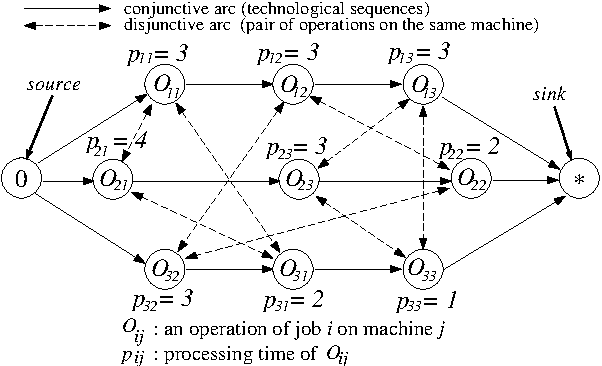
\includegraphics[width=0.8\linewidth]{images/jssp_disjunctive_graph.pdf}\\
    Figure 1.2: Disjunctive graph representation of, retrieved from \cite{YamadaNakanoJSSP}
\end{center}
